
\newpage
\section{GN2X: GN2 Variant for Boosted Higgs Decays to Heavy Flavours}\label{app-chap-GN2X}
This section presents an interesting application of the \gls{gn2} architecture to a specialised objective: identifying boosted Higgs boson decaying into a pair of $b$- or $c$-quarks. Having an effective tagger to identify these boosted decays can significantly help analyses studying the decay of Higgs particles to a $c\bar{c}$ pair \cite{ATLAS:2022ers}, for the precise measurement of the Higgs boson $p_T$ spectrum \cite{PhysRevD.105.092003}, and for beyond the \gls{sm} measurements \cite{ATLAS:2023azi}. To perform this task, a new algorithm labelled GN2X is introduced based on the design of \gls{gn2} \cite{ATL-PHYS-PUB-2023-021}. Its main task is to discriminate jets from boosted Higgs boson decaying into a $b\bar{b}$ or a $c\bar{c}$ pair from those originating from the fully-hadronic top-quark decay and the multi-jet processes. While other taggers presented in this chapter relied on small-radius ($R=0.4$) PFlow jets or \gls{vr} jets, GN2X is trained on jet reconstructed with a large-radius ($R=1.0$) with \gls{ufo} objects to capture the majority of the decay products \cite{atlasLARGERJet}. \gls{ufo} combines PFlow \cite{atlasPFLOW} and Track-Calo clusters objects \cite{ATL-PHYS-PUB-2017-015}, thereby including neutral and charged components in the reconstruction. \gls{ufo} large-$R$ jets are reconstructed with the anti-$k_T$ algorithm with a radius $R = 1.0$ \cite{Cacciari:2008gp}. \\

To train the algorithm, Higgs produced in association with a $Z$-boson and decaying to a pair of heavy flavour quarks ($b\bar{b}$ or a $c\bar{c}$) are simulated. To not bias the result towards a specific $p_T$, $\eta$, and mass distributions of the jets, the simulations are resampled to have an approximately flat distribution of jet mass in the training set, while the validation set follows the \gls{sm} $ZH$ production for a Higgs boson $H$ of a mass equal to 125 GeV. Similarly, the top-quark decay with subsequent hadronic decay of the $W$ boson in the $t \rightarrow bW$ chain is simulated for the training samples using a hypothetical $Z'$-boson of 4 TeV mass decaying as $Z' \rightarrow t\bar(t)$ with approximately flat jet $p_T$ distribution. The evaluation sample uses the \gls{sm} $t\bar{t}$ decay with filters on the scalar sum of the objects $p_T$ in the event. Finally, the multi-jet process is simulated in slices of particle-level jet $p_T$ to have the same spectrum. More details on the simulated samples used can be found in Ref. \cite{ATL-PHYS-PUB-2023-021}. After resampling the samples to enforce the same $p_T$, $\eta$, and mass distributions, there are 62 million jets split between 15 million $H_{b\bar{b}}$, 15 million $H_{c\bar{c}}$, 10 million top, and 22 million multi-jets. \\

The previous algorithm for this task that now serves as benchmark in this study is the $X_{bb}$ tagger, a feed-forward network combining the flavour tagging discriminants of \gls{dl1r} or \gls{dl1d} for up to three \gls{vr} sub-jets associated to the large-$R$ jet \cite{ATL-PHYS-PUB-2020-019, ATL-PHYS-PUB-2021-035}. The track selection is similar to that of the GN-models (Section \ref{chap:GN}), and the inputs of the model are equivalent to those of Table~\ref{tab:gnInputVariables}, with the jet variables defined on the large-$R$ jet with the addition of the mass of the large-$R$ jet. At most 100 tracks associated with a jet are supplied to the network, as sorted by the decreasing transverse impact parameter significance $S_{d_0}$. The same auxiliary tasks as in \gls{gn2} are used with the same respective weights and neural network designs. The initialiser has a 192 embedding dimension and the transformer encoder combines 6 layers with 4 attention heads. The global representation is again obtained from an attention-weighted sum over the conditional tracks, with learnable attention weights. GN2X contains in total 1.5 million parameters and is trained on 4 A100 \glspl{gpu} for 40 epochs ($\sim$1 hour per epoch) with a batch size of 1000. \\

The model outputs four probabilities $p_{H_{b\bar{b}}}$, $p_{H_{c\bar{c}}}$, $p_{\textrm{top}}$, and $p_{\textrm{QCD}}$ that are combined in a discriminant score equivalent to Equations \ref{bdisc} and \ref{cdisc}: 
\begin{equation}
  D_{H_{b\bar{b}}} = \log \frac{p_{H_{b\bar{b}}}}{f_{H_{c\bar{c}}} . p_{H_{c\bar{c}}} + f_{\textrm{top}} . p_{\textrm{top}} + (1 - f_{H_{c\bar{c}}} - f_{\textrm{top}}) . p_{\textrm{QCD}}},
\end{equation}
where the flavour fractions were chosen from dedicated performance studies to be $f_{H_{c\bar{c}}} = 0.02$ and $f_{\textrm{top}} = 0.25$. A discriminant for $H_{c\bar{c}}$ is similarly defined with $f_{H_{b\bar{b}}} = 0.3$ and $f_{\textrm{top}} = 0.25$:
\begin{equation}
  D_{H_{c\bar{c}}} = \log \frac{p_{H_{c\bar{c}}}}{f_{H_{b\bar{b}}} . p_{H_{b\bar{b}}} + f_{\textrm{top}} . p_{\textrm{top}} + (1 - f_{H_{b\bar{b}}} - f_{\textrm{top}}) . p_{\textrm{QCD}}}.
\end{equation}

The performance of GN2X can be assessed from the \gls{roc} curves presented in Figure~\ref{fig:rocGN2X}. An additional performance to $X_{bb}$ and GN2X is presented, where two individual \gls{vr} sub-jets are $b$- or $c$-tagged by a \gls{vr}-trained \gls{gn2} model. The jets used are the leading \gls{vr} sub-jets associated with the large-$R$ jet. Note that $X_{bb}$ was not retrained on the specific samples but uses the \gls{vr}-trained \gls{dl1d} previously introduced. A clear performance gained is delivered by the GN2X method above both the $X_{bb}$ tagger and the combination of two individual tags with \gls{gn2}. The latter approach does not access correlations between the sub-jets, explaining its lower performance at higher $H(b\bar{b})$ and $H(c\bar{c})$ efficiencies than the GN2X and $X_{bb}$ model. At a 50\% $H(b\bar{b})$ \gls{wp}, GN2X improves the top rejection (multi-jet rejection) on $X_{bb}$ by a factor 1.6 (2.5) \cite{ATL-PHYS-PUB-2023-021}. For $H(b\bar{b})$ tagging, the $H(c\bar{c})$ background is negligible. GN2X also improves the performance for $H(c\bar{c})$ tagging over the approach combining two individual \gls{vr} tagged-jets: at a 50\% \gls{wp}, GN2X improves the top rejection by a factor 3, the multi-jet rejection by a factor 5, and the $H(b\bar{b})$ rejection by a factor 6. This novel approach to perform boosted object tagging is the first of its kind in ATLAS and is now integrated into the ATLAS software.

\begin{center}
  \begin{figure}[h!]
  \centerline{
  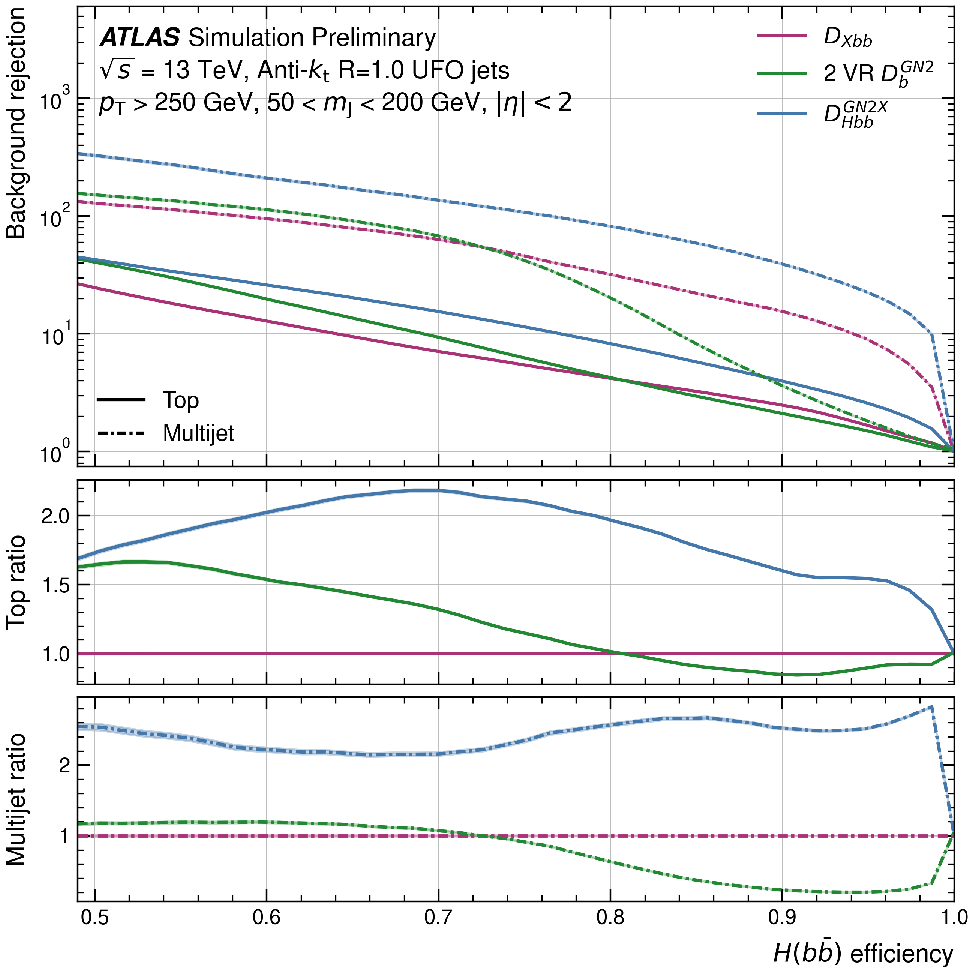
\includegraphics[width=0.50\textwidth]{Images/FTAG/GN2X/roc/rocHbb.pdf}
  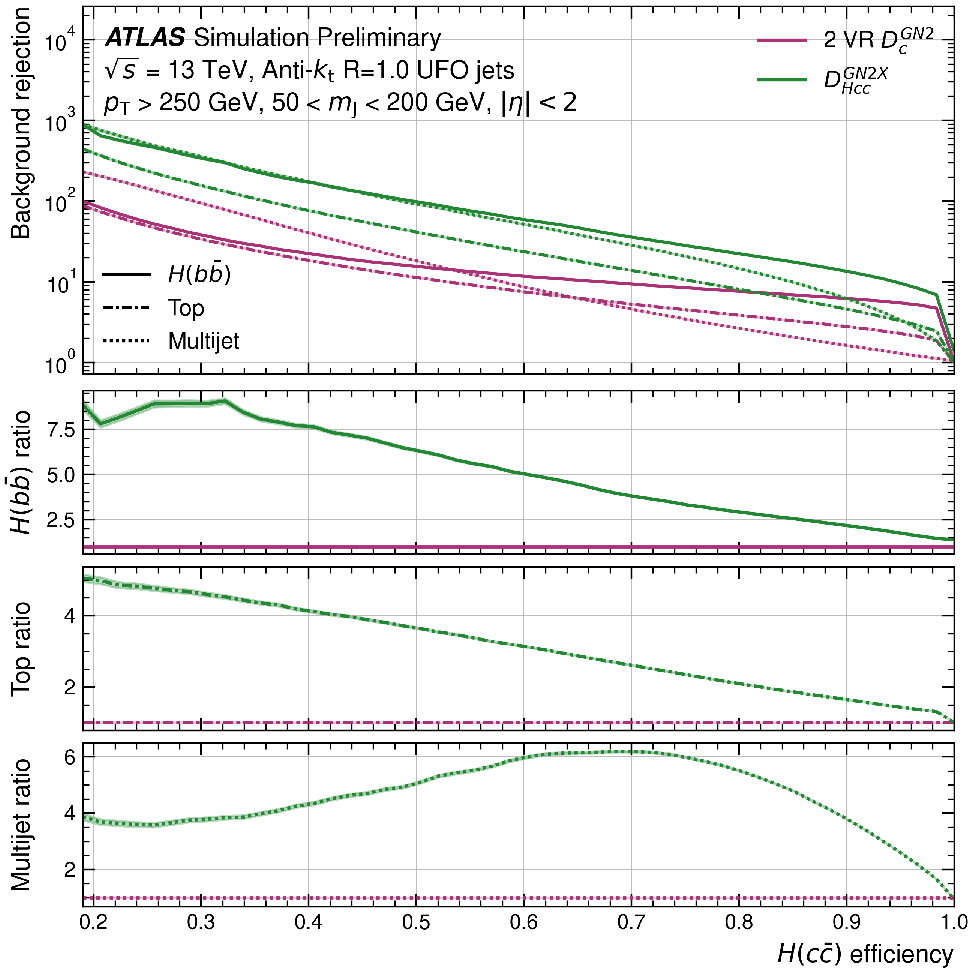
\includegraphics[width=0.50\textwidth]{Images/FTAG/GN2X/roc/rocHcc.pdf}
  }
  \caption{The ROC curves for $H(b\bar{b})$ (left) and $H(c\bar{c})$ tagging (right) on an SM simulated test samples \cite{ATL-PHYS-PUB-2023-021}. The respective tagging efficiency is displayed versus the top and multi-jet rejections, for jets with a $p_T > 250$ GeV and a mass $50 < m_J < 200$ GeV. Models compared are the baseline $X_{bb}$ tagger, using the variable-radius DL1r of at most 3 identified sub-jets in the large-$R$ jet, the tag obtained by combining the tag on two variable-radius jets within the large-$R$ jet with the single-jet GN2 tagger, and the GN2X model. The former is only available for $H(b\bar{b})$ tagging, and the $H(b\bar{b})$ rejection is displayed for $H(c\bar{c})$ tagging. The $H(c\bar{c})$ background is negligible for $H(b\bar{b})$ tagging. Shaded regions represent the binominal error band.}
  \label{fig:rocGN2X}
  \end{figure}
\end{center}